%%%%%%%%%%%%%%%%%%%%%%%%%%%%%%%%%%%%%%%%%
% Professional Mathematical Presentation Template
% 
% This template uses the beamer class with the Madrid theme
% and a custom color scheme for a clean, professional look
% that works well with mathematical content.
%%%%%%%%%%%%%%%%%%%%%%%%%%%%%%%%%%%%%%%%%

\documentclass[aspectratio=169]{beamer} % 16:9 aspect ratio (modern)

% Theme settings
\usetheme{Madrid}
\usecolortheme{default}


\definecolor{primcolor}{RGB}{25,50,100} % Dark blue
\setbeamercolor{structure}{fg=primcolor}
\setbeamercolor{frametitle}{bg=primcolor!15, fg=primcolor}
\setbeamercolor{title}{fg=white} % White title text for contrast
\setbeamercolor{subtitle}{fg=white} % White subtitle text
\setbeamercolor{author}{fg=primcolor} % White author text
\setbeamercolor{date}{fg=primcolor} % White date text
\setbeamercolor{institute}{fg=primcolor} % White institute text

% Font settings
\usefonttheme{professionalfonts}
\usefonttheme{serif}

% Package imports
\usepackage{amsmath, amsfonts, amssymb, amsthm} % Math packages
\usepackage{mathtools} % Enhanced math tools
\usepackage{bm} % Bold math symbols
\usepackage{graphicx} % For images
\usepackage{booktabs} % Professional tables
\usepackage{tikz} % For diagrams
\usetikzlibrary{arrows, positioning, matrix, decorations.pathreplacing}

% Use beamer's theorem styles
\setbeamertemplate{theorem}[ams style]
\setbeamertemplate{theorems}[numbered]


% Remove navigation symbols
\setbeamertemplate{navigation symbols}{}

% Custom footer
\setbeamertemplate{footline}{
  \leavevmode%
  \hbox{%
  \begin{beamercolorbox}[wd=.333333\paperwidth,ht=2.25ex,dp=1ex,center]{author in head/foot}%
    \usebeamerfont{author in head/foot}\insertshortauthor
  \end{beamercolorbox}%
  \begin{beamercolorbox}[wd=.333333\paperwidth,ht=2.25ex,dp=1ex,center]{title in head/foot}%
    \usebeamerfont{title in head/foot}\insertshorttitle
  \end{beamercolorbox}%
  \begin{beamercolorbox}[wd=.333333\paperwidth,ht=2.25ex,dp=1ex,right]{date in head/foot}%
    \usebeamerfont{date in head/foot}\insertshortdate{}\hspace*{2em}
    \insertframenumber{} / \inserttotalframenumber\hspace*{2ex} 
  \end{beamercolorbox}}%
  \vskip0pt%
}

% Title information
\title[DL]{Reading Note of Deep Learning solution to DSGE models}
\subtitle{Pascal et al 2024}
\author[Longye]{Longye Tian \\ \texttt{longye.tian@anu.edu.au}}
\institute[ANU]{Australian National University\\ School of Economics}
\date{April 1st, 2025}
\DeclareFontFamily{U}{mathx}{\hyphenchar\font45}
\DeclareFontShape{U}{mathx}{m}{n}{
      <5> <6> <7> <8> <9> <10>
      <10.95> <12> <14.4> <17.28> <20.74> <24.88>
      mathx10
      }{}
\DeclareSymbolFont{mathx}{U}{mathx}{m}{n}
\DeclareMathSymbol{\bigtimes}{1}{mathx}{"91}

\begin{document}

% Title frame
\begin{frame}
  \titlepage
\end{frame}

% Outline frame
\begin{frame}{Outline}
  \tableofcontents
\end{frame}

\section{The Approximation Problem - A generic AI problem}
\begin{frame}{A generica AI problem}
    A generic AI problem is approximating an unknown function
$$
F^*: \mathbb{R}^m \to \mathbb{R}^n
$$
using
\begin{itemize}
    \item potentially noisy observations of inputs $x\in\mathbb{R}^m$
    \item and output $y = F^*(x)\in\mathbb{R}^n$
\end{itemize}
\end{frame}

\begin{frame}{Some concepts}
\begin{itemize}
    \item Let the \textbf{candidate set}
    $$
    S = \{F(\cdot; \theta): \theta\in \mathbb{R}^p\}
    $$
    denote a set of \textbf{known} functions indexed by the vector of parameters $\theta$
    \item Let $L:\mathbb{R}^n\times \mathbb{R}^n\to \mathbb{R}$ denote a loss function penalizing approximation errors, i.e.,
    
    $$L[F(x,\theta), y]$$ 
    measures the cost associated with a discrepancy between the prediction $F(x,\theta)$ and the actual output $y$.
    \item Let $P:\mathbb{R}^m\times \mathbb{R}^n\to \mathbb{R}_+$ denote the joint cumulative distribution function of $(x, y)$.
\end{itemize}
    
\end{frame}

\begin{frame}{Solution concept}
To solve the approximation problem over $S$ is to \textbf{find the parameter vector $\theta^*$} such that
$$
\theta^* = \arg\min_{\theta}\,\, \textcolor{blue}{\Xi(\theta)}
$$
where the \textcolor{blue}{expected approximation error} is
$$
\Xi(\theta):= \int L[F(x,\theta ),y]\,\textcolor{red}{\underbrace{dP(x,y)}_{\text{unknown}}} = \mathbb{E}\{L[F(x,\theta),y]\}
$$

    
\end{frame}

\begin{frame}{Conditions needed to solve the problem }
\begin{itemize}
    \item Candidate set $S$ must be flexible enough to contain functions close to $F^*$ -- Otherwise, underfitting
    \item We are able to replace the unknown objective function $\Xi(\theta)$ by a valid approximation 
    \item We are able to perform the actual minimization.
\end{itemize}
    
\end{frame}

\begin{frame}{What DL offers}

\begin{itemize}
    \item Candidate set $S$ must be flexible enough to contain functions close to $F^*$ -- Otherwise, underfitting \textcolor{red}{--> Neural Network}
    \item We are able to replace the unknown objective function $\Xi(\theta)$ by a valid approximation \textcolor{red}{-->empirical counterpart}
    \item We are able to perform the actual minimization. \textcolor{red}{-->gradient descent}
\end{itemize}

\end{frame}

\section{The objective function}

\begin{frame}{The Objective Function - Empirical Counterpart}
\begin{itemize}
    \item Minizing the expected loss $\Xi(\theta)$ is not feasible in practice because the joint distribution of inputs and outputs is unknown.
    \item Invoke the standard laws of large number to build an accurate estimate of the objective function. 
\end{itemize}
    
\end{frame}

\begin{frame}{LLN to estimate the objective function}
    Let $\{(x_i,y_i)\}_{i=1}^n$ denote a sample of $n$ independent observations on inputs and outputs. Then the \textbf{empirical cost}
    $$
    \widehat{\Xi}_n(\theta) = \frac{1}{n}\sum_{i=1}^n L[F(x_i;\theta),y_i]
    $$
    provides an \textbf{unbiased and consistent} estimate of $\Xi(\theta)$.
\end{frame}

\begin{frame}{Choice of Loss functions}
Loss function $L$ quantifies the discrepancy between model-implied outputs and actual observations. \textbf{Its choice is model dependent}
\begin{itemize}
    \item a continuous loss function might work well when the output is a real number
    \item a different loss function might work well when the output is binary
    \item In Maliar et al 2021 JMP, they cast the economic model in DL form using a regression representation in which $F$ outputs a real number. A natural loss function in this case is the mean squared error.
\end{itemize}
    
\end{frame}

\section{Artificial neural networks}

\begin{frame}{Neuron}
The basic unit of neural networks are called \textbf{neuron/nodes/perceptron/unit}. 
\begin{itemize}
    \item It is a simple function
    $$
    g: \mathbb{R}^k \to \mathbb{R}
    $$
    \item take a vector $z\in\mathbb{R}^k$ as input
    \item transform it using an \textbf{affine mapping}
    \item parameterized by a vector of \textbf{weights} $\gamma\in\mathbb{R}^{k+1}$.
    \item applies a non-linear function (\textbf{activation function}) $f$ to output a real number.
\end{itemize}
    
\end{frame}


\begin{frame}{Neuron}
    The basic unit of neural networks are called \textbf{neuron/nodes/perceptron/unit}. 
\begin{itemize}
    \item It is a simple function
    $$
    g: \mathbb{R}^k \to \mathbb{R}
    $$
\end{itemize}
Formally,

$$
g(z;\gamma) = f\left(\underbrace{\gamma_0}_{\text{bias}} + \sum_{i=1}^k \gamma_i z_i\right)
$$
\end{frame}

\begin{frame}{Layer}
A \textbf{layer} with $p$ nodes is a vector function stacking $p$ neurons, i.e.,
$$
G:\mathbb{R}^k \to \mathbb{R}^p
$$
or
$$
G(z;\Gamma)  = \begin{bmatrix}
    g(z;\gamma_1)\\
    \cdots\\
    g(z;\gamma_p)
\end{bmatrix},\quad \text{where $\Gamma = (\gamma_1, \gamma_2,\cdots, \gamma_p)$}
$$

We call it a layer with \textbf{width $p$}.\\
\\
\textcolor{blue}{\textbf{Remark}: In this presentation, we assume that all neurons in a layer share the same input and same activation function. It can be more sophisticated.}
\end{frame}

\begin{frame}{Neural network/neural net/multilayer perception}
    A \textbf{neural network} is a composition of several layers. Let $G_1,\cdots, G_\ell$ denote $\ell$ layers of conformable dimensions. A neural network is a function
    $$
    N:\mathbb{R}^m \to \mathbb{R}^n
    $$
    $$
    N(x) = (\underbrace{G_\ell}_{output} \circ \underbrace{G_{\ell-1} \circ \cdots\circ G_2}_{hidden}\circ \underbrace{G_1}_{input})(x)
    $$

    \begin{itemize}
        \item we call the number of layer $\ell$ the \textbf{length of neural net}
        \item we call the largest width of layers the \textbf{width of neural net}
    \end{itemize}
    \textcolor{blue}{\textbf{Remark}: Only the input and output layers are contrained by the dimensions of the variable of interest. Hidden layers are not}
\end{frame}
\begin{frame}{Deep Neural Nets}
Deeper neural nets are more flexible and have the potential learn more complex function.
    \begin{itemize}
        \item More than three layers $\implies$ deep
        \item Less than three layers $\implies$ shallow 
    \end{itemize}
\end{frame}

\begin{frame}{Universal Approximation Theorem}
A neural network can approximate any continuous function from one-dimensional space to another with any desired non-zero amount of error, provided it is given sufficient depth or sufficient width.
    
\end{frame}

\begin{frame}{Curse of dimensionality}
For a given approximation error, the number of parameters required to approximate a function with a neural network increase \textbf{linearly with the dimension} of the input $x$, while it increases exponentially for most other classes of approximators.
    
\end{frame}
\begin{frame}{Robustness}
Neural networks are robust to
\begin{itemize}
    \item multi-collinearity
    \item various kinks
    \item discontinuities
\end{itemize}
    
\end{frame}

\begin{frame}{Problem}
\begin{itemize}
    \item Universal Approximation Theorem do not specify how to identify the neural net with the best fit
    \item No gurantee neural nets can actually learn the function, i.e., identify the loss-minizing value of $\theta$ given the amount of available data.
\end{itemize}
    
\end{frame}

\begin{frame}{Design of Neural Network}
Three choices involving design a neural net
\begin{itemize}
    \item activation function 
    \item Width
    \item Depth
\end{itemize}
    
\end{frame}

\begin{frame}{Activation Functions}
\begin{itemize}
    \item Introduce nonlinearity in the algorithm 
    \item All universal approximation theorem needs nonlinear activation function
    \item We need smooth activation functions to use gradient descent
    \item logistic sigmoid and hyperbolic tangent vanish fast when away from the origin, makes the gradient descent algoritm slow--> vanishing gradient problem
    \item ReLu has two numerical advantage: sparse activation, efficient computation, use leaky ReLU for gradient non-zero almost everywhere
    \item Use ReLu as benchmark for input and hidden layers
\end{itemize}
    
\end{frame}

\begin{frame}{Output activation function}
    \begin{itemize}
        \item unconstrained output $\implies$ identity function
        \item non-negative output $\implies$ exponential function
        \item probability $\implies $ Sigmoid and Softmax
    \end{itemize}
\end{frame}

\begin{frame}{Depth and Width}
Two rules of thumb
\begin{itemize}
    \item Deeper neural net works typically require far fewer neurons per layer, and therefore far fewer parameters, they tend to generalize better. 
    $\implies$
    a deeper neural network are preferable to wider network
    \item Complexity of NN should be adapted to the complexity of the approximation problem.
\end{itemize}
    
\end{frame}

\begin{frame}{Gradient Descent}
    \begin{itemize}
        \item The gradient of a differentiable function 
        $$
        G:\mathbb{R}^m \to \mathbb{R}
        $$
        indicates the local direction of steepest ascent
        \item So
        $$
        G(x+\lambda x) -G(x)
        $$
        is maximized in the neighborhood of $x\in\mathbb{R}^m$, i.e., for $\lambda >0$ small
        \item 
        $$
        v = \nabla G(x)
        $$
        is the gradient of $G$ evaluated at $x$
        \item Conversely
        $$
        G(x+\lambda x) -G(x)
        $$
        is locally minimized by moving the direction opposite to the gradient, i.e., steepest descent.
    \end{itemize}
\end{frame}

\begin{frame}{Gradient of the empirical loss}
    $$
    \widehat{\Xi}_n(\theta) = \frac{1}{n}\sum_{i=1}^n L[F(x_i;\theta),y_i]
    $$
    Gradient of the empirical loss is
    $$
    \nabla \widehat{\Xi}_n(\theta) = \frac{1}{n} \sum_{i=1}^n\nabla_\theta L[F(x_i,\theta),y_i]
    $$
    \begin{itemize}
        \item Each evaluation of the gradient requires a full pass through the dataset --> batch learning -- consider the full batch of data before updating the parameter $\theta$
    \end{itemize}
\end{frame}


\begin{frame}{Stochastic gradient descent algorithm}
\begin{figure}
    \centering
    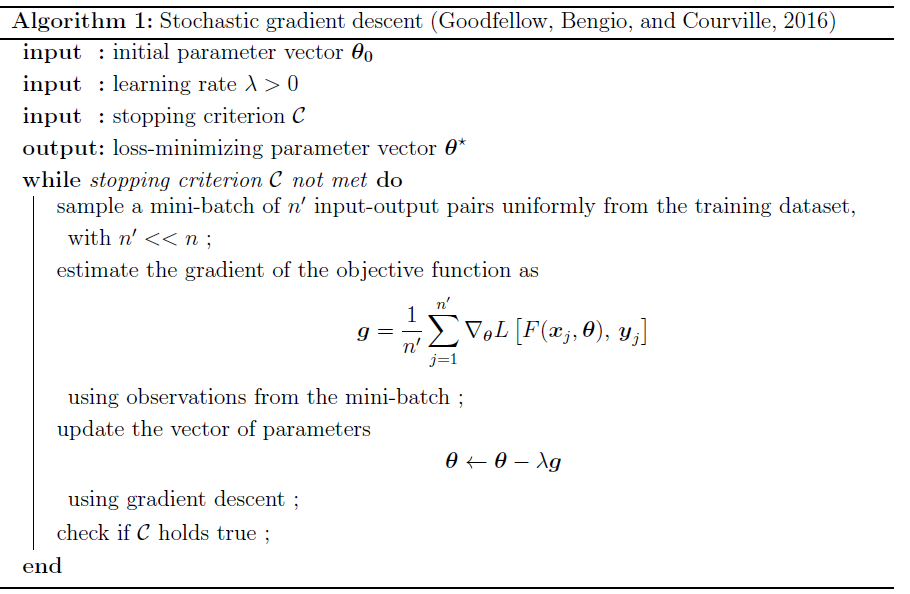
\includegraphics[width=0.7\linewidth]{DL on Macro model/Pascal et al 2024 Working paper/Reading Note/stochastic gradient descent algorithm.png}

\end{figure}
    
\end{frame}

\begin{frame}{Validation and Regularization}
The overall objective of DL technique is to provide algorithm that perform well on new inputs

\begin{itemize}
    \item Don't underfit: able to identify and learn the important properties of the data from the traning sample
    \item Don't overfit: not learned various idiosyncrasies of the training dataeset that will not generalize well to new inputs
    \item Broaderly: model should have the right capacity for the task force, i.e., the complexity is enough to represent the data but not overly complex. ==> the NN should have the right structure. This is validation
\end{itemize}
    
\end{frame}








\end{document}
